\documentclass[aspectratio=169]{beamer}
\usetheme[block=fill]{metropolis}
\usepackage{tikz}
\usetikzlibrary{shapes.geometric, arrows.meta, positioning, calc}

\title{Building a Reproducible Scholarly Search Toolkit}
\subtitle{Episode 4: The Normalized Document \& Author Model}
\author{Scholar Search Kit}
\date{}

\begin{document}

\begin{frame}[plain]
  \titlepage
\end{frame}

\begin{frame}{Episode Goal}
  \begin{alertblock}{The Goal}
    Create the core \texttt{Document} and \texttt{Author} dataclasses to serve as the universal language of our system.
  \end{alertblock}
  \vspace{0.5cm}
  Every provider (OpenAlex, arXiv, Crossref) returns wildly different JSON. We must map them all into a single, strongly-typed \texttt{Document} structure immediately upon ingest.
\end{frame}

\begin{frame}{The Normalization Boundary}
  \begin{center}
  \resizebox{0.75\linewidth}{!}{
  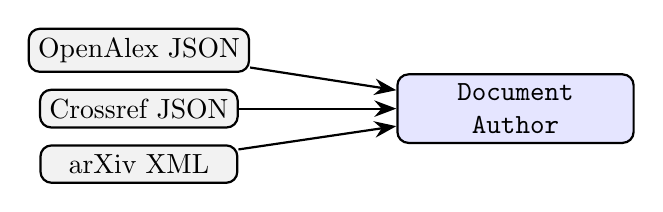
\begin{tikzpicture}[
      node distance=1.5cm and 2cm,
      provider/.style={rectangle, draw, thick, rounded corners, minimum width=2.5cm, align=center, fill=black!5},
      model/.style={rectangle, draw, thick, rounded corners, minimum width=3cm, align=center, fill=blue!10},
      arrow/.style={-{Stealth[scale=1.2]}, thick}
    ]
    
    \node[provider] (openalex) {OpenAlex JSON};
    \node[provider, below=0.2cm of openalex] (crossref) {Crossref JSON};
    \node[provider, below=0.2cm of crossref] (arxiv) {arXiv XML};
    
    \node[model, right=of crossref] (document) {\texttt{Document}\\\texttt{Author}};
    
    \draw[arrow] (openalex) -- (document);
    \draw[arrow] (crossref) -- (document);
    \draw[arrow] (arxiv) -- (document);
  \end{tikzpicture}
  }
  \end{center}
\end{frame}

\begin{frame}{The \texttt{Document} Model}
  \begin{block}{Key Fields}
    Enforcing strict types prevents runtime crashes during analysis.
  \end{block}
  
  \begin{itemize}
      \item \texttt{external\_ids}: Our \texttt{ExternalIds} object.
      \item \texttt{title} \& \texttt{abstract}: Text content.
      \item \texttt{authors}: List of \texttt{Author} objects.
      \item \texttt{year} \& \texttt{publication\_date}: For temporal filtering.
      \item \texttt{provider\_id}: Provenance (e.g., "openalex").
  \end{itemize}
\end{frame}

\begin{frame}{Implementation: UTC Timestamps}
  \begin{block}{The Golden Rule of Time}
    Always store dates and times in UTC.
  \end{block}
  
  \begin{itemize}
      \item We add a \texttt{retrieved\_at} field to track exactly when we pulled this data.
      \item This guarantees auditability—essential for systematic literature reviews where search dates matter.
  \end{itemize}
\end{frame}

\begin{frame}{Verification}
  \begin{alertblock}{Success Criteria}
    \begin{itemize}
        \item Can instantiate a \texttt{Document} with mocked data.
        \item Missing required fields trigger \texttt{TypeError}.
        \item \texttt{Author} objects correctly nest inside the \texttt{Document}.
    \end{itemize}
  \end{alertblock}
\end{frame}

\end{document}
